\documentclass[french, 11pt]{article}
\usepackage[utf8]{inputenc}
\usepackage[T1]{fontenc}
\usepackage[a4paper]{geometry}
\usepackage{lmodern}
\usepackage{xcolor}
\usepackage{graphicx}
\usepackage{textcomp}
\usepackage[french]{babel}
\usepackage[breaklinks]{hyperref}
\usepackage{colortbl}


% Title Page
\title{Cahier des charges\\ Space Wars}
\date{Date de rédaction: 7 Juin 2016}
\author{Tony Deborguere \\ Baris Tekeli \\ Malik Touat \\ Qi Zhiwen}

% mails
% -----

\begin{document}
	\maketitle
	\begin{center}
		
\includegraphics[width=0.5\linewidth]{alien}
	\end{center}
	\newpage
	\begin{center}
	\end{center}
	\newpage
	
	\tableofcontents
	
	\newpage
	
		
	\section{Présentation}
		\begin{table}[h]
			\begin{center}
				\centering
				\begin{tabular}{llr}
					\hline\hline
					\rowcolor[RGB]{125,12,125}\multicolumn{3}{c}{\textcolor{white}{Fiche d'identité du projet}}\\\hline\hline
					Nom du projet: & Space Wars &\\\hline
					Objet: & \multicolumn{2}{l}{Création d'un clone de Space Invaders avec une partie Player}\\
					& Versus Player.&\\\hline
					Membres du projet: & DEBORGUERE TONY & (t.deborguere@gmail.com) \\ %%%%% à finir
					&TEKELI BARIS & (tekelibaris@gmail.com) \\
					&TOUAT MALIK & (mal.touat@gmail.com) \\
					&QI ZHIWEN & (531940615@qq.com) \\\hline
					Commanditaire: & JULIEN DEHOS &\\\hline
					Date de début: & 06 Juin 2016 &\\\hline
					Date de fin: & 24 Juin 2016 &\\\hline
				\end{tabular}
			\end{center}
		\end{table}
		
		Ce projet a était retenu puisqu'il nous permet d’avoir un affichage graphique simple et facilement reconnaissable.
		De plus, si le temps nous le permet, une évolution dans ce domaine est envisageable.
		La partie PVP\footnote{Abréviation de Player Versur Player} permettra l’ajout des éléments réseaux.
\newpage
	\section{Définition des besoins}
		
		\subsection{Contexte général}
		Dans le cadre de notre fin d’année, nous avons était approché par Mr. Julien Dehos, pour lui
		développer un nouveau jeu.
		Il souhaite avoir un jeu qui dispose d’une interface graphique capable d’être jouer en réseaux avec des amis.
		Pour la partie graphique, la bibliothèques multimédia nommée \og{}SFML\footnote{\label{SFML}Simple and Fast Multimedia Library}\fg{} nous est imposée.
		Il ne manifesta pas d’intérêt particulier sur le choix
		du jeu mais précisa qu’il devait être fonctionnel.
		
		\subsection{Besoins et priorités}
		Les deux besoins évoqués par le client sont:
		\begin{description}
			\item[Besoin 1] Possibilité de jouer en réseaux.
			\begin{itemize}
				\item Soit en tour par tour.
				\item Soit en temps réel.
			\end{itemize}
			\item[Besoin 2] Une interface graphique (avec la bibliothèque SFML\ref{SFML}).
		\end{description}

		L’interface se doit d’être clair et simple d’utilisation pour l’utilisateur, et devra faire l’objet
		d’un développement soigné pour ne pas nuire au jeu.
		L’aspect le plus important est bien évidement le fait que le jeu soit fonctionnel avant la date de fin du projet, même si cela implique de sacrifier certaines fonctionnalités.
		
		\newpage
		\section{Règle du jeu}
		Space Wars est un clone de Space Invaders: un jeu d'arcade. Le principe est de détruire des vagues d'aliens au moyen d'un missile en se déplaçant horizontalement sur l'écran. Ce jeu fait parti des classiques du jeu vidéo au même titre que Pac-Man et d'autres de ses contemporains.
		\\
		\begin{itemize}
			\item Le jeu commence avec un vaisseau qui a 3 points de vie et une vague de $5 * 11$, soit 55 aliens.
			\item Le joueur, qui incarne le vaisseau, a la possibilité de se déplacer uniquement à l'horizontal.
			\item Le vaisseau tire des laser très rapide.
			\item Un seul laser du vaisseau peu être présent sur la carte à la fois, ce qui veut dire que pour tirer un laser, le précédent doit être détruit.
			\item La vague d'ennemis se déplace horizontalement et descend petit à petit.
			\item Si la vague descend au point de toucher le vaisseau, alors celui-ci perd 1 point de vie et la vague remonte de 3 lignes.
			\item Si le joueur atteint 0 point de vie, la partie est terminée.
			\item Entre la vague et le vaisseau, il y a 4 boucliers.
			\item Les boucliers seront détruits petit à petit après chaque impact avec un missile (adverse ou allié).
			\item Les missiles du vaisseau vont uniquement de bas en haut, et ceux de l'ennemi de haut en bas. Les missiles progressent uniquement verticalement et ne peuvent être déviés.
			\item Les missiles ennemis peuvent être détruits avec un missile du vaisseau.
			\item Un alien touché par un missile se voit détruit avec celui-ci.
			\item Chaque alien détruit donne un malus à l'adversaire (sauf en jeu solo) et rapporte des points de score, selon le type d'alien.
			\item Il y a 4 types d'aliens:
			\begin{itemize}
				\item Type 1: Alien tirant un laser peu rapide.
				\item Type 2: Alien tirant un laser rapide.
				\item Type 3: Alien tirant un laser très rapide 
				\item Type 4: Alien très rapide bonus inoffensif raportant 200 points. 
			\end{itemize}
			\item La vague est constituée de :
			\begin{itemize}
				\item 1\ier{} et 2\ieme{}~rang: type 1 \textrightarrow~10 points.
				\item 3\ieme{} et 4\ieme{}~rang: type 2 \textrightarrow~20 points.
				\item 5\ieme{}~rang: type 3 \textrightarrow~50 points.
			\end{itemize}
			\item Si le vaisseau est touché par un missile, le vaisseau perd 1 point de vie et le missile est détruit.
			\item Si un alien est derrière un autre alien, seul celui qui est devant peut tirer.
			\item A la fin de la partie, le perdant aura un malus pour la partie d'après. (sauf en jeu solo).
		\end{itemize}
		\subsection{Conditions de victoire}\label{conditionsDeVictoire}
		\begin{itemize}
			\item Détruire tous les aliens sur la carte.
		\end{itemize}
		
		\section{Spécifications}
			\begin{itemize}
				\item Logiciel fonctionnant sous les distribution linux (Debian \& Basée sur Debian).
				\item Création et Gestion d’un Menu avec une interface graphique.
				\begin{description}
					\item L'utilisateur peut se déplacer dans le menu avec les flèches directionnelles du clavier et sélectionne ce qu'il souhaite faire avec la touche entrer.
				\end{description}
				\item Fonctionnalités de choix du type de jeu:
				\begin{itemize}
					\item Fonctionnalités d’un jeu Solo.
					\begin{description}
						\item Le joueur joue une partie seul, obtient un score et peut recommencer s'il le souhaite après la fin de la partie.
						\item Le score est enregistré après chaque fin de partie.
					\end{description}					
					\item Fonctionnalités d’un jeu JcJ\footnote{Joueur contre Joueur, équivalent français du Player vs Player}.
					\begin{description}
						\item Le joueur joue une partie contre un autre joueur en réseaux. La partie se termine quand l'un des deux meurt ou élimine tous les aliens.
					\end{description}
					\item Fonctionnalités d’un jeu JcO\footnote{Joueur contre Ordinateur.}.
					\begin{description}
						\item Le joueur joue une partie contre l'intelligence artificielle. La partie se termine quand l'un des deux meurt ou élimine tous les aliens.
					\end{description}
				\end{itemize}
				\item Fonctionnalités de gestion d’une partie :
				\begin{itemize}
					\item Définir les conditions de victoire.
					\begin{description}
						\item Vous retrouverez les conditions de victoire ici: \ref{conditionsDeVictoire}
					\end{description}
					\item Fonctionnalités de déplacement avec le clavier.
					\begin{description}
						\item[Flèche du droite] Se déplacer à droite.
						\item[Flèche du gauche] Se déplacer à gauche.
					\end{description}
					\item Fonctionnalités de Tir avec le clavier.
					\begin{description}
						\item[Barre d'espace] Tirer un missile.
					\end{description}
					\item Fonctionnalités d’impact.
					\begin{description}
						\item Quand il y a un impact, le missile qui est l'élément A est détruit, et des dégâts sont causés à l'élément B.
					\end{description}
				\end{itemize}
				\item Fonctionnalités Réseaux :
				\begin{itemize}
					\item Connexion Client / Serveur.
					\begin{itemize}
						\item Le client se connecte au serveur.
						\item Le serveur attend la connexion d'un deuxième client sur le même port pour lancer une partie en réseaux.
						\item Lors d'une partie en tour par tour:
						\begin{itemize}
							\item A la fin de la partie en cours, le score du premier joueur est enregistré, et le second doit battre le score du premier.	
						\end{itemize}
						\item Lors d'une partie en temps réel:
						\begin{itemize}
							\item La partie se termine dès qu'un des joueurs atteint 0 points de vie ou qu'ils éliminent tous les aliens de la carte.
							\item Celui qui a le meilleur score après la fin de la partie gagne.
							\item Un malus est envoyé au joueur 1 à chaque fois qu'un alien est détruit par le joueur 2, et vise versa.
						\end{itemize}
					\end{itemize}
				\end{itemize}
				\item Fonctionnalité d’intelligence artificiel. (Optionnel)
				\begin{description}
					\item[IA] Une intelligence artificielle qui permet de jouer à Space Wars.
				\end{description}
				\item Interface utilisateur :
				\begin{description}
					\item Affichage Simple respectant l’aspect graphique de Space Invaders.
					\item Gestion du plein écran.
				\end{description}
			\end{itemize}
			\newpage
			\section{Annexe}
			\subsection{Livrables}
			\begin{itemize}
				\item Logiciel déployé sur la machine du client.
				\item Code source documenté sous licence \og GNU– GPL v35 \fg{}.
				\item Script d’installation et de compilation (Makefile) .
				\item Manuel d’utilisation.
				\item Fichier ReadMe.
			\end{itemize}
			\subsection{Diagramme de cas d'utilisation}
			\begin{figure}[h]
				\centering
				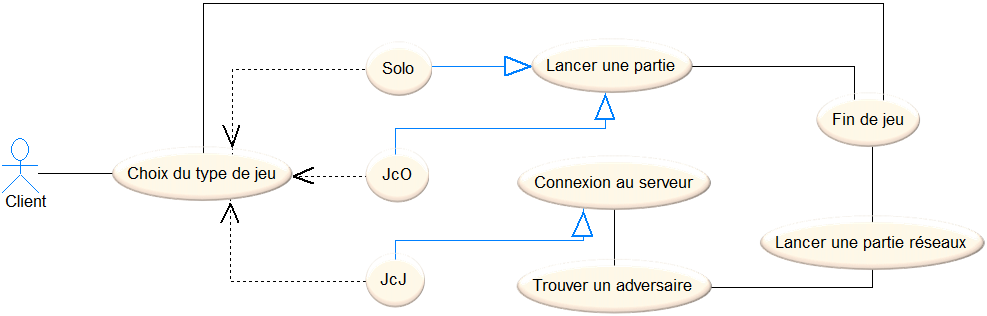
\includegraphics[width=1\linewidth]{DiagrammeDeCasDutilisation2}
				\caption{Diagramme de cas d'utilisation}
			\end{figure}
			\newpage
			\subsection{Diagramme de classe}
			\begin{figure}[h]
				\centering
				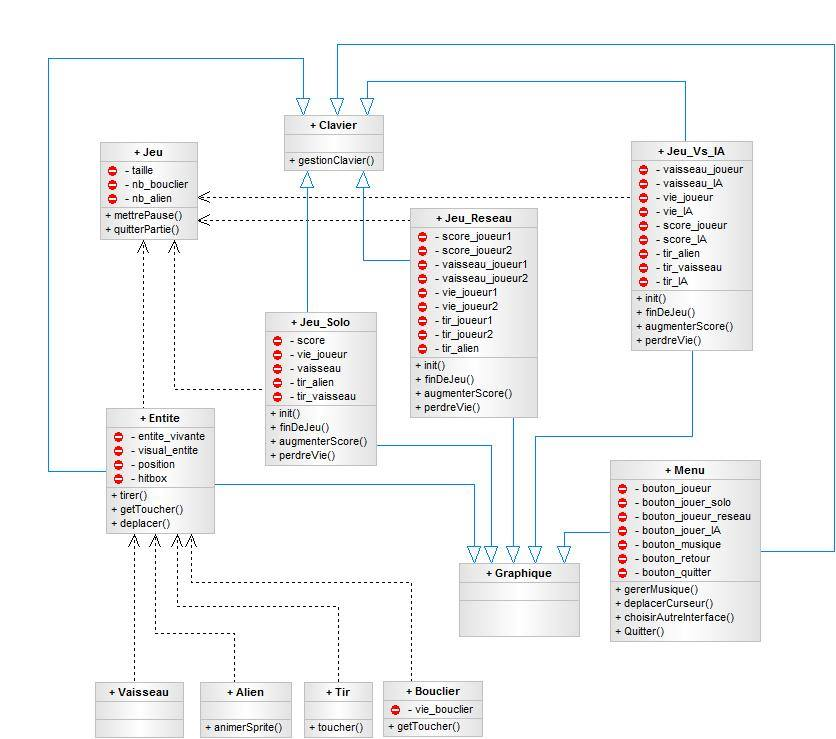
\includegraphics[width=1\linewidth]{DiagrammeDeClasse}
				\caption{Diagramme de classe}
			\end{figure}
			\newpage
			\subsection{Maquettes}
			
			\begin{table}[h]
				\begin{center}
					\centering
					\begin{tabular}{cc}
						Maquette menu & Maquette jeu \\
						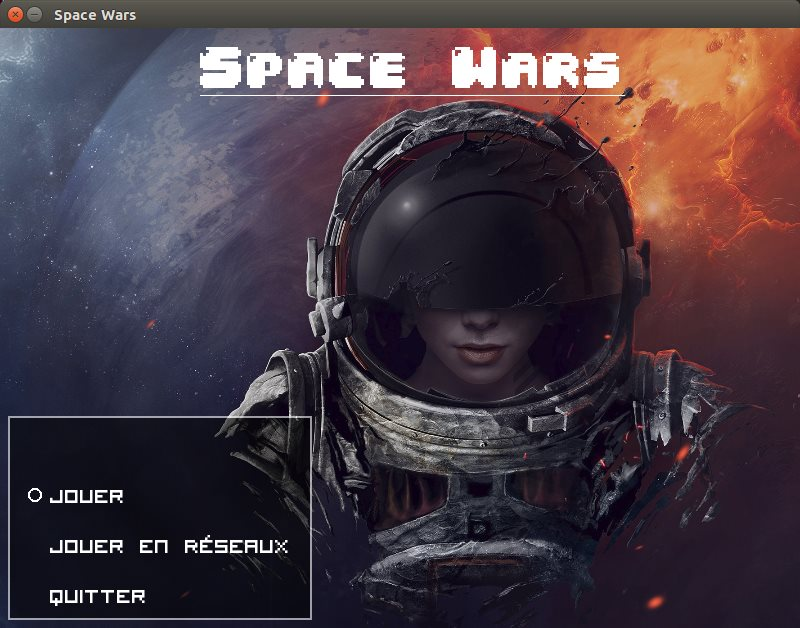
\includegraphics[width=0.5\linewidth]{Maquette1}
						&
						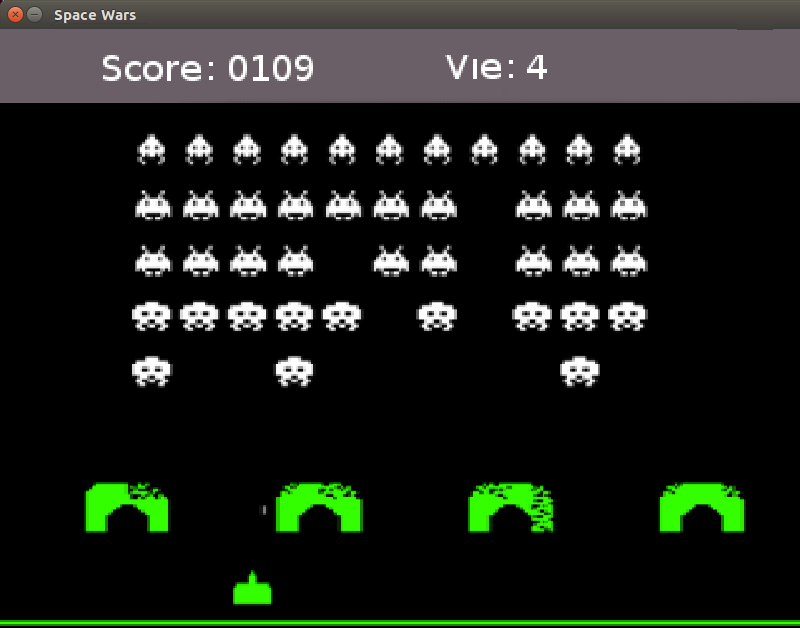
\includegraphics[width=0.5\linewidth]{Maquette2} \\
						&\\&\\
						\multicolumn{2}{c}{Maquette réseaux} \\
						\multicolumn{2}{c}{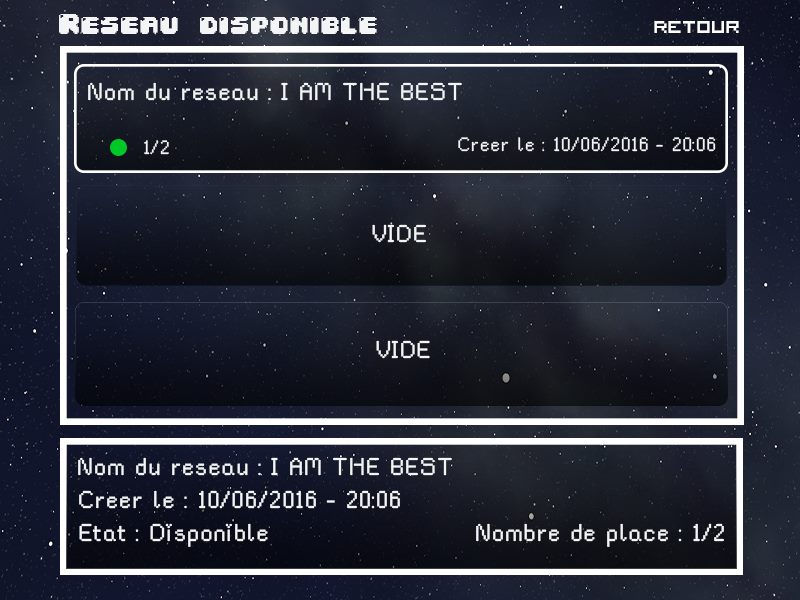
\includegraphics[width=0.5\linewidth]{MaquetteReseaux}}\\
					\end{tabular}
				\end{center}
			\end{table}
			\newpage
			\subsection{Planning prévisionnel}
			\begin{figure}[h]
				\centering
				\includegraphics[width=1.05\linewidth]{PlanningPrévisionnelPng}
				\caption{Planning prévisionnel}
			\end{figure}
\end{document}          
